\documentclass[12pt]{article}
\usepackage[a4paper]{geometry}
\usepackage[myheadings]{fullpage}
\usepackage{fancyhdr}
\usepackage{lastpage}
\usepackage{graphicx, wrapfig, subcaption, setspace, booktabs}
\usepackage[T1]{fontenc}
\usepackage[font=small, labelfont=bf]{caption}
\usepackage{fourier}
\usepackage[protrusion=true, expansion=true]{microtype}
\usepackage[spanish]{babel}
\usepackage{sectsty}
\usepackage{url, lipsum}
\usepackage{hyperref}
\usepackage{fancyhdr,lipsum}


\hypersetup{
    colorlinks=true, %set true if you want colored links
    linktoc=all,     %set to all if you want both sections and subsections linked
    linkcolor=blue,  %choose some color if you want links to stand out
}
\urlstyle{same}


\newcommand{\HRule}[1]{\rule{\linewidth}{#1}}
\onehalfspacing

\setcounter{secnumdepth}{2}
\setcounter{tocdepth}{5}

%-------------------------------------------------------------------------------
% HEADER & FOOTER
%-------------------------------------------------------------------------------
\pagestyle{fancy}
\fancyhf{}
\setlength\headheight{15pt}
\fancyhead[L]{SSII}
\fancyhead[R]{\uppercase{Instalación de Sistemas Operativos}}
\fancyfoot[R]{Page \thepage\ of \pageref{LastPage}}

%-------------------------------------------------------------------------------
% TITLE PAGE
%-------------------------------------------------------------------------------

\begin{document}

\title{ \normalsize \textsc{SISTEMAS INFORMÁTICOS\\
I.E.S FRANCISCO DE LOS RÍOS}
		\\ [2.0cm]
		\HRule{0.5pt} \\
		\LARGE \textbf{\uppercase{Instalación de Sistemas Operativos}}
    \HRule{0.5pt} \\
    \HRule{2pt} \\ [0.5cm]
    %\normalsize  \vspace*{10\baselineskip}
    \LARGE \textbf{\uppercase{WINDOWS 10}}
    \HRule{2pt} \\ [0.5cm]
    \normalsize  \vspace*{2\baselineskip}
    }

\author{
        Trabajo realizado por: \\
		Antonio Muñoz Cubero
	    \normalsize  \vspace*{4\baselineskip}
		}
\date{\textbf{01 de Febrero de 2021}}
\newpage
\maketitle
\newpage

%-------------------------------------------------------------------------------
% Table of Content
\tableofcontents
\newpage
%-------------------------------------------------------------------------------

%-------------------------------------------------------------------------------
% Section title formatting
\sectionfont{\scshape}
%-------------------------------------------------------------------------------






%-------------------------------------------------------------------------------
% BODY
%-------------------------------------------------------------------------------


    \section*{Introducción}
      En el transcurso de esta práctica seguiremos los pasos adecuados para que la Instalación del sistema 
      operativo, en este caso \textbf{Windows 10} se realice de manera satisfactoria. También hemos de cumplir 
      una serie de criterios para la correcta realización de la misma, que son los siguientes.
      \begin{itemize}
        \item Se realizará la configuración del hardware virtual según los requisitos del sistema invitado 
        (memoria RAM y tamaño de disco) para ello se buscará información en la página Web de Microsoft 
        para consultar cuáles son dichos recursos mínimos.
        \item  El nombre del sistema o del usuario en su defecto (durante la instalación) será igual al nombre 
        de usuario del alumno/a en moodle. (Captura de pantalla).
        \item Omitir la creación de cuenta en Microsoft mediante correo electrónico (Captura de pantalla).
        \item La conexión de red será de tipo NAT o Red NAT con configuración IP automática.
        \item Una vez instalado comprobar que el sistema está actualizado, pero no instalar las actualizaciones. 
        (Captura de pantalla).
      \end{itemize}
      También he de destacar que la imagen que usaré para la instalación del sistema operativo fue proporcionada por el 
      profesor.

    \newpage
    
    \section{Creacion de la máquina virtual}
      El primer paso de esta práctica es la creación y configuración de una máquina virtual adecuada para la instalación 
      del sistema operativo que vayamos a utilizar, en nuestro caso usaremos \textbf{Windows 10}. Para ello, abrimos 
      nuestro programa de virtualización y le damos a añadir una nueva máquina virtual y nos desplegará el siguiente menú
      en el caso que usemos \textit{virtual box}
      \begin{figure}[h]
        \centering
        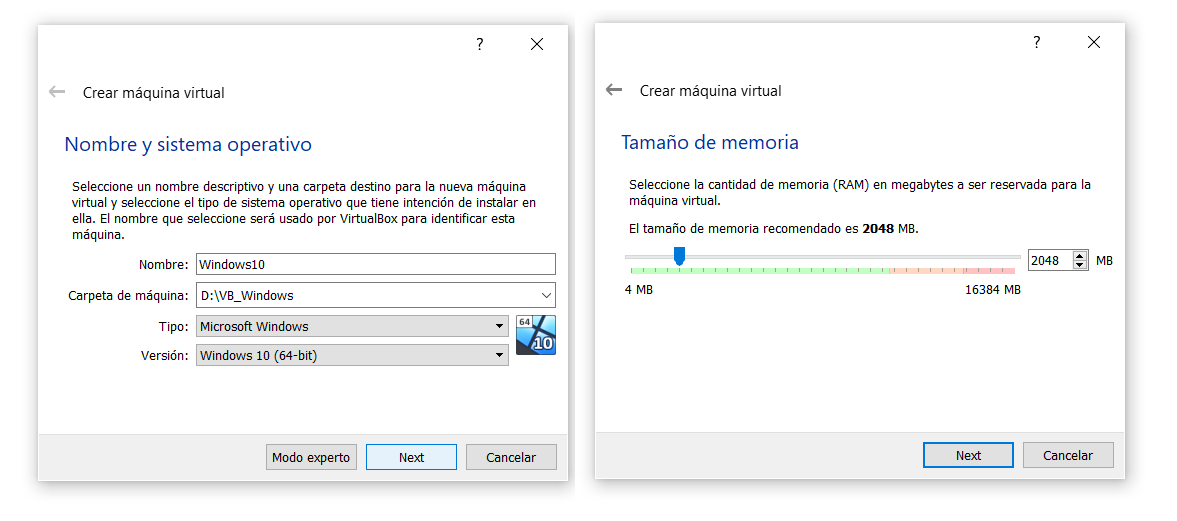
\includegraphics[scale = 0.5]{img/windows_install_1.png}
        \caption{Creacion de la máquina virtual.}
        \label{Windows1}
      \end{figure}

      La configuración de la máquina virtual está hecha acorde a los requisitos mínimos del sistema, que previamente hemos 
      buscado. Tras esto, solo hemos de confirar la máquina virtual siguiendo dichos requisitos.

      \begin{figure}[h]
        \centering
        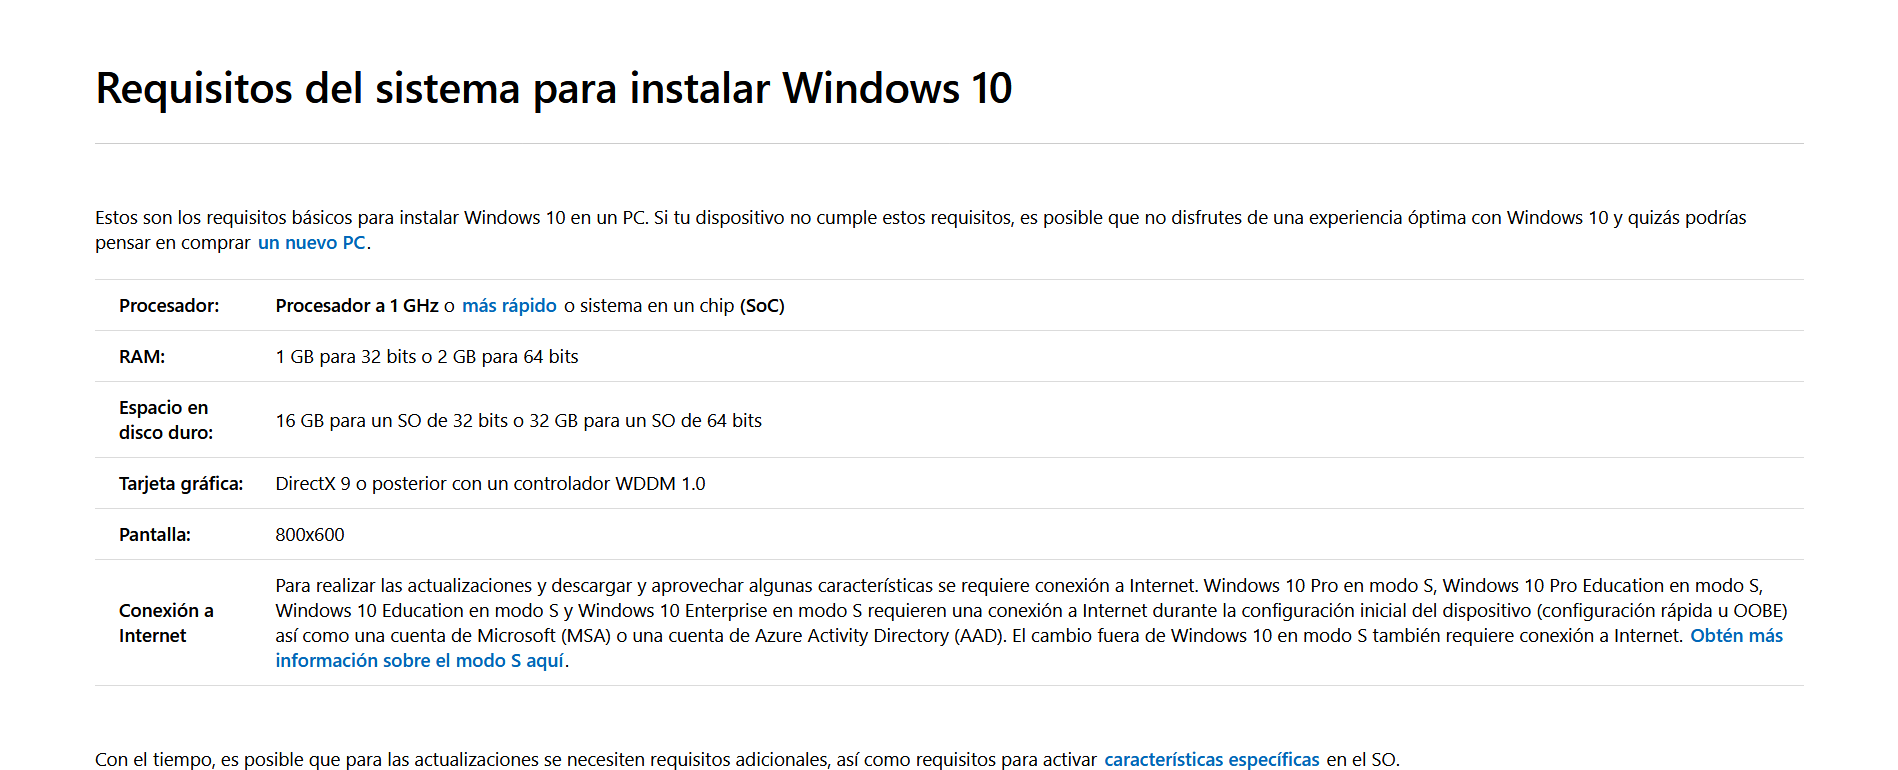
\includegraphics[scale = 0.4]{img/requisitos_w10.png}
        \caption{Requisitos mínimos Windows 10.}
        \label{requisitos}
      \end{figure}

      \newpage

      Ahora simplemente, rellenamos los campos que nos piden con los parámetros adecuados para el correcto 
      funcionamiento del sistema.

      \begin{figure}[h]
        \centering
        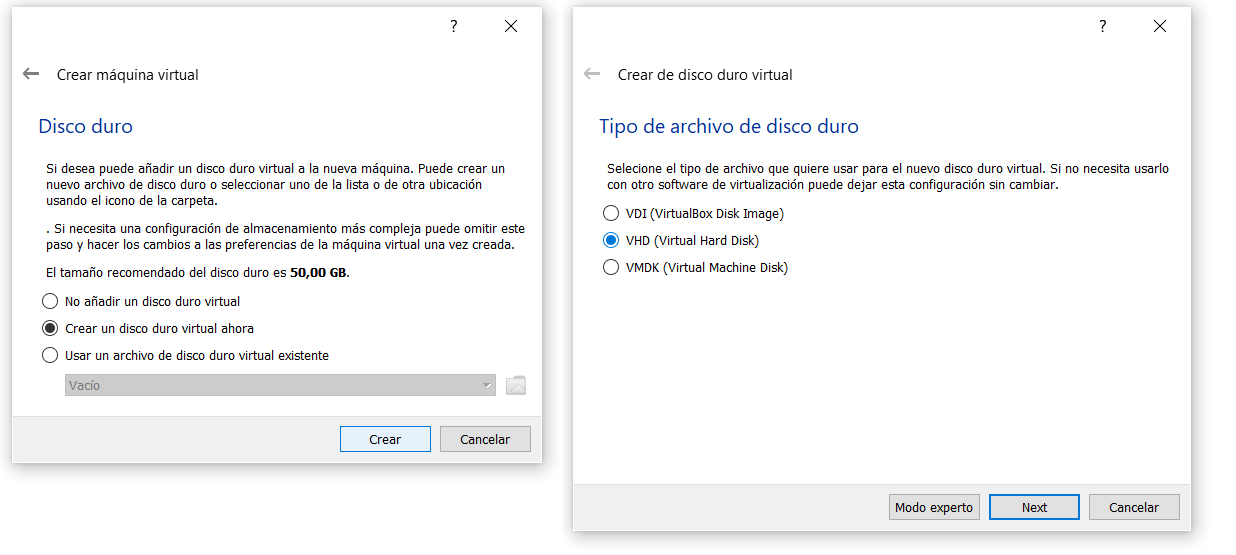
\includegraphics[scale = 0.5]{img/windows_install_3.png}
        \caption{Creacion de la máquina virtual.}
        \label{Windows2}
      \end{figure}

      \begin{figure}[h]
        \centering
        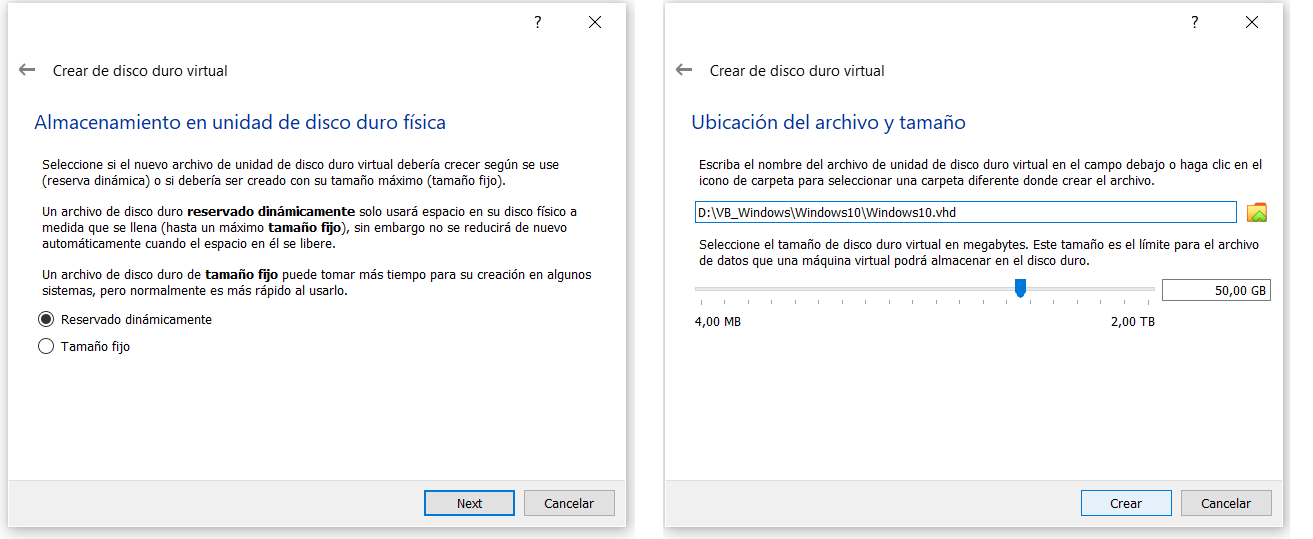
\includegraphics[scale = 0.5]{img/windows_install_5.png}
        \caption{Creacion de la máquina virtual.}
        \label{Windows3}
      \end{figure}
    
      Una vez seguidos estos pasos, nuestra máquina virtual estará creada y lista para su funcionamiento. Ahora 
      nos queda montar la imagen y proceder a la instalación.
    
      \newpage

    \section{Instalación de Windows 10}

      El siguiente paso a seguir es la instalación del propio sistema operativo, para ello, arracamos la máquina 
      virtual que acabamos de crear y nos pedirá que seleccionemos un disco de inicio.

      \begin{figure}[h]
        \centering
        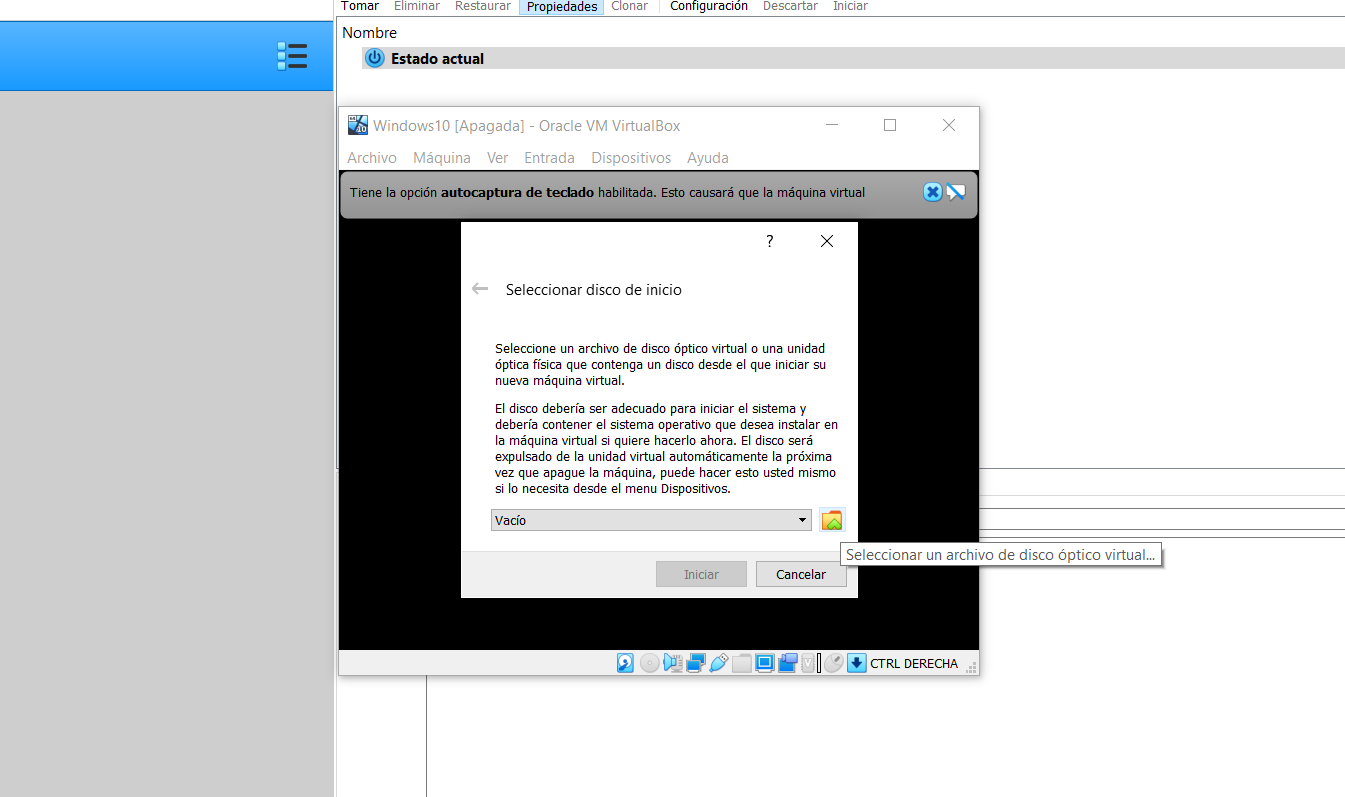
\includegraphics[scale = 0.35]{img/windows_install_8.png}
        \caption{Selección del disco de inicio.}
        \label{Windows4}
      \end{figure}

      En este apartado seleccionamos la ubicación del archivo \textit{.iso} que hemos descargado previamente y 
      continuamos pulsando \textit{Iniciar}.

      Nos pedirá que seleccionemos los idiomas tanto del sistema a instalar como del teclado que estamos usando y
      el formato de fecha y hora de nuestra zona. 

      \begin{figure}[h]
        \centering
        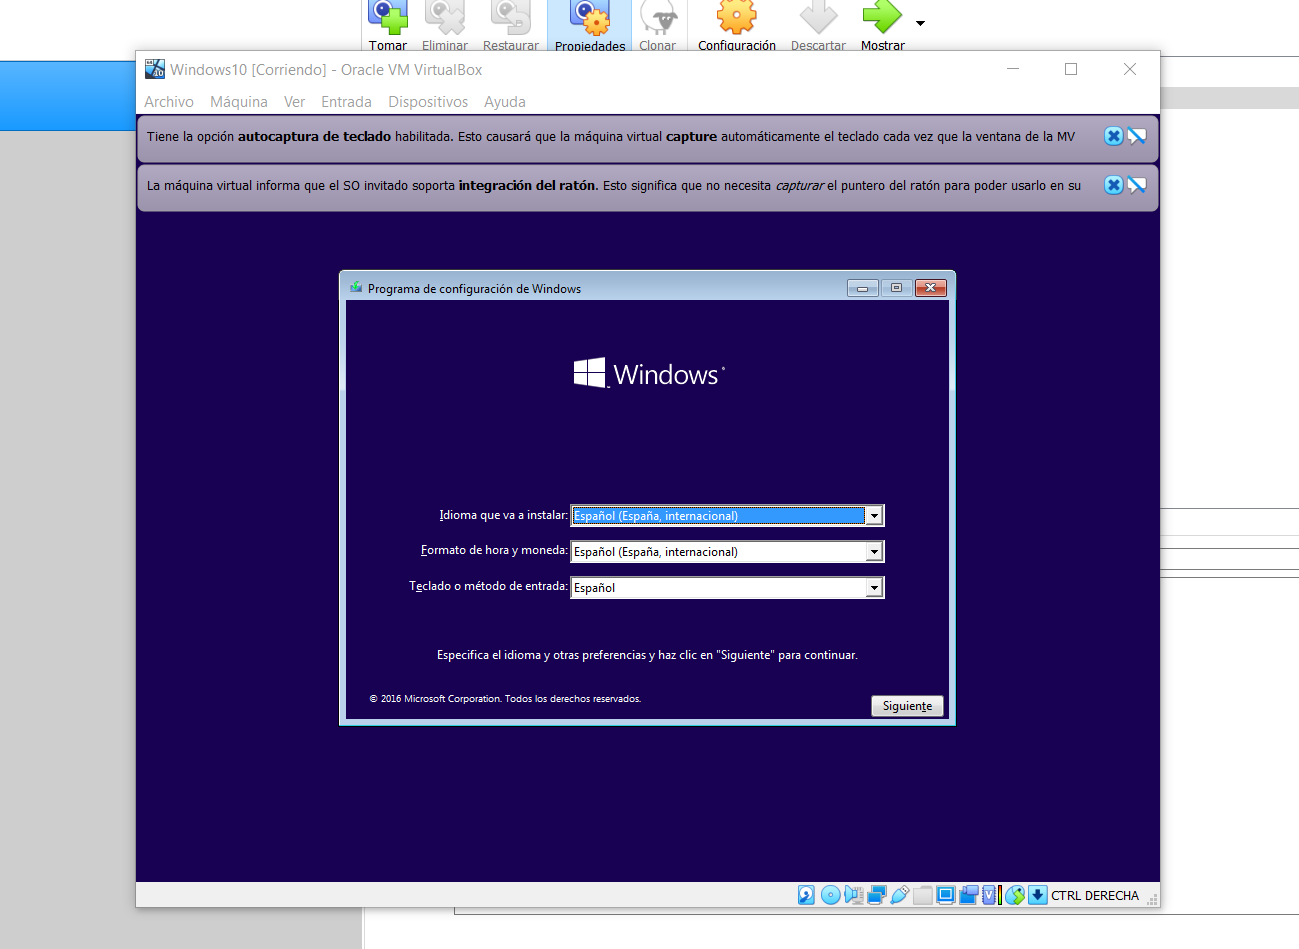
\includegraphics[scale = 0.35]{img/windows_install_9.5.png}
        \caption{Selección de idiomas.}
        \label{Windows5}
      \end{figure}
    
      \newpage

      Una vez seleccionado el idioma y pasado a la siguiente fase pulsando en instalar, tardará un periodo prolongado 
      hasta que requiera de nuestras acciones, como en el caso de que nos pide un \textbf{código de licencia de Windows.}
      
      \begin{figure}[h]
        \centering
        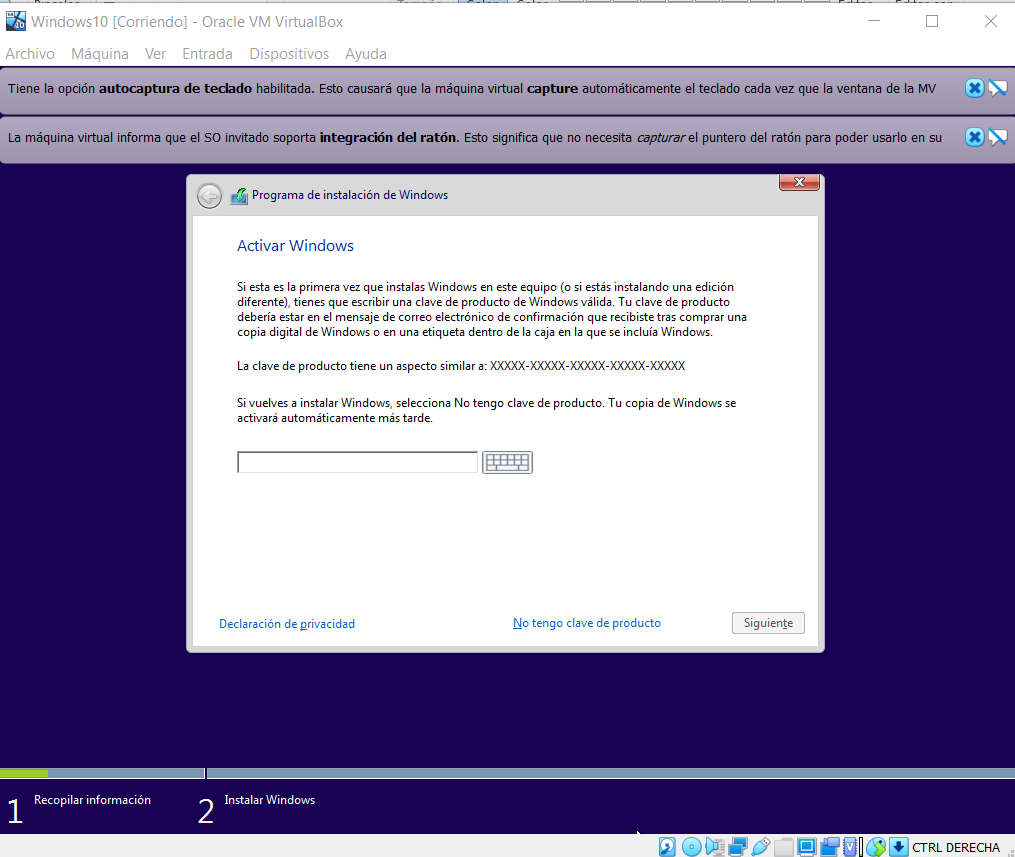
\includegraphics[scale = 0.5]{img/windows_install_11.png}
        \caption{Introducir código de activación.}
        \label{Windows6}
      \end{figure}

      En nuestro caso no pondremos ninguno y pulsaremos \textit{No tengo clave del producto}, puesto que no vamos a sacar 
      nada a producción y lo usamos con fines educativos, en caso de que estemos instalando Windows en una máquina para 
      nuestro uso diario o profesional, debemos de introducir una licencia.
      \\\\
      El siguiente punto en la instalación es la elección entre si instlar el sistema \textit{Windows 10 pro} o \textit{Windows 10 home}.
      En mi caso instalaré el \textbf{pro}.
      \begin{figure}[h]
        \centering
        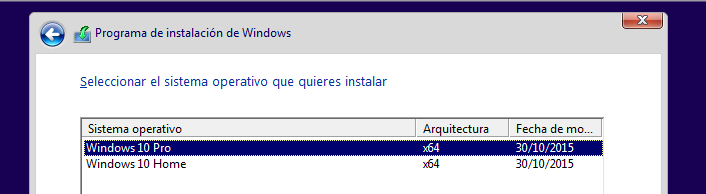
\includegraphics[scale = 0.7]{img/windows_install_12.png}
        \caption{Elección de versión.}
        \label{Windows7}
      \end{figure}
      
      \newpage

      En la siguiente ventana de nuestra instlación nos darán a elegir dos opciones que son las siguientes:

      \begin{figure}[h]
        \centering
        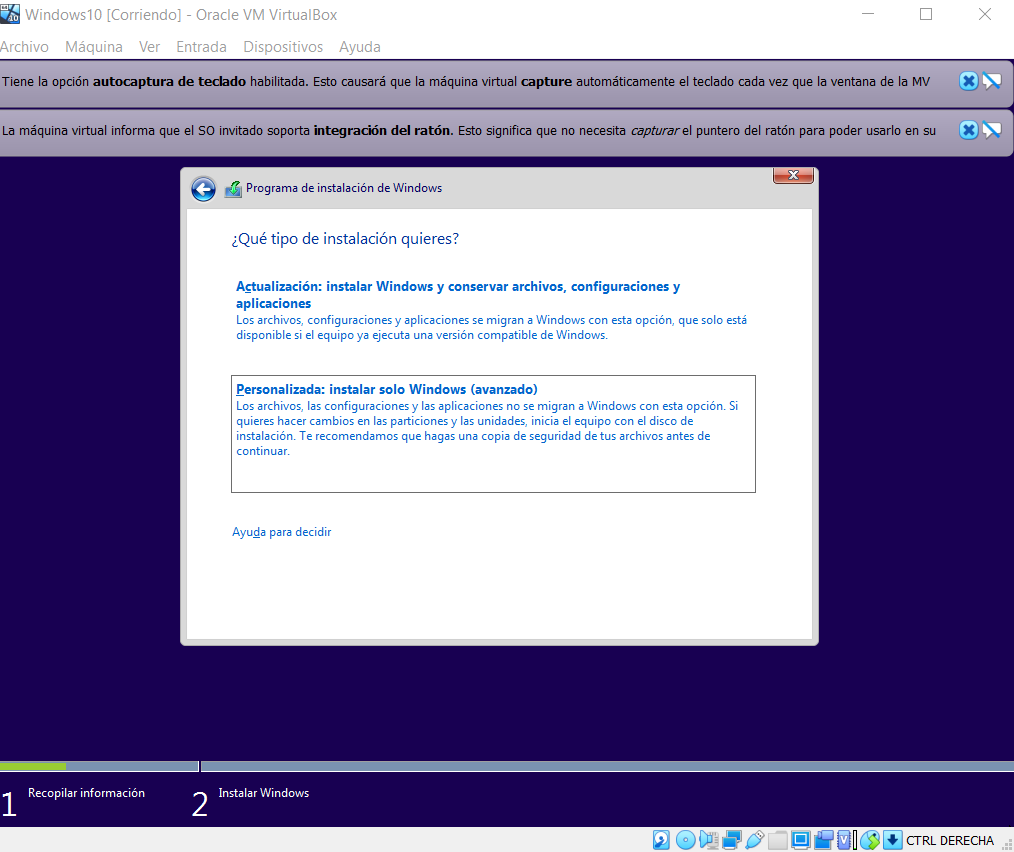
\includegraphics[scale = 0.4]{img/windows_install_13.png}
        \caption{Elección de instalación.}
        \label{Windows8}
      \end{figure}

      En la opción de \textit{Personalizada}, más adelante podremos elegir una serie de opciones que nos permetirar 
      prescindir de una serie de características del software que pueden ser algo engorrosas para el usuario, y hará 
      el sistema mas liviano. Pero lo veremos más adelante. Seguidamente seleccionamos el disco donde deseemos instalar 
      el sistema operativo para continuar con la instalación.

      \begin{figure}[h]
        \centering
        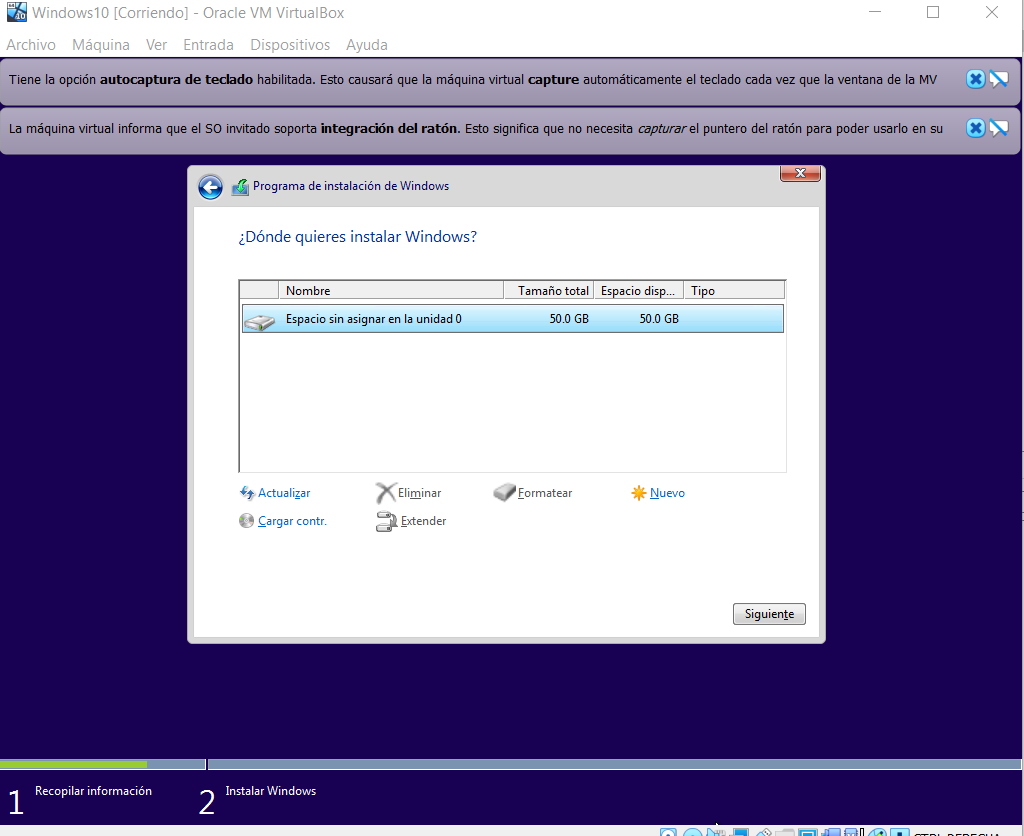
\includegraphics[scale = 0.4]{img/windows_install_14.png}
        \caption{Selección de disco.}
        \label{Windows9}
      \end{figure}
    
      \newpage

      Ahora el proceso que se inicia es el de instalación del sistema operativo, puede tardar bastante, por tanto hay que 
      tener paciencia.\\
      Una vez acabada la instalación se reiniciará el equipo y pasaremos a tener Windows 10 instalado satisfactoriamente.\\
      Nos saldrá una ventana que nos dirá si queremos realizar la configuración de una serie de opciones de forma manual o de 
      manera rápida.

      \begin{figure}[h]
        \centering
        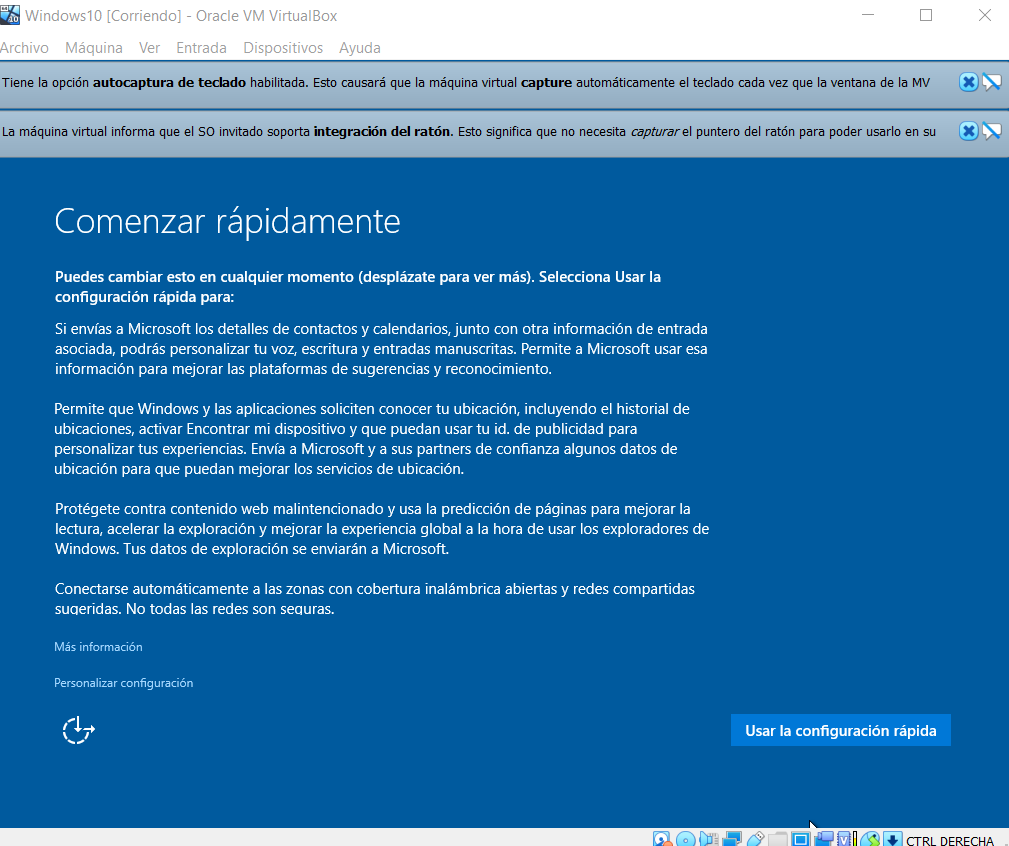
\includegraphics[scale = 0.5]{img/windows_install_16.png}
        \caption{Elección de configuración.}
        \label{Windows10}
      \end{figure}

      Si lo haceis de forma manual podréis desactivar todos los servicios que proveen a Microsoft de información sobre vuestro 
      computador, lo recomendable es desactivarlas manualmente pulsando en \textit{Personalizar configuración}.
      \\\\
      Una vez desactivadas todos los apartados que nos mostraba o elegida la opción de configuración rápida, pasamos a la siguiente 
      funcionalidad de Windows 10.

      \newpage

      En la siguiente ventana el configurador nos pedirá un correo de una cuenta Microsoft, es importante no introducir ninguno previamente 
      puesto que después si es necesario se puede iniciar sesión, pero por ahora es mejor prescindir de ello. pulsando en \textit{Omitir este paso.}

      \begin{figure}[h]
        \centering
        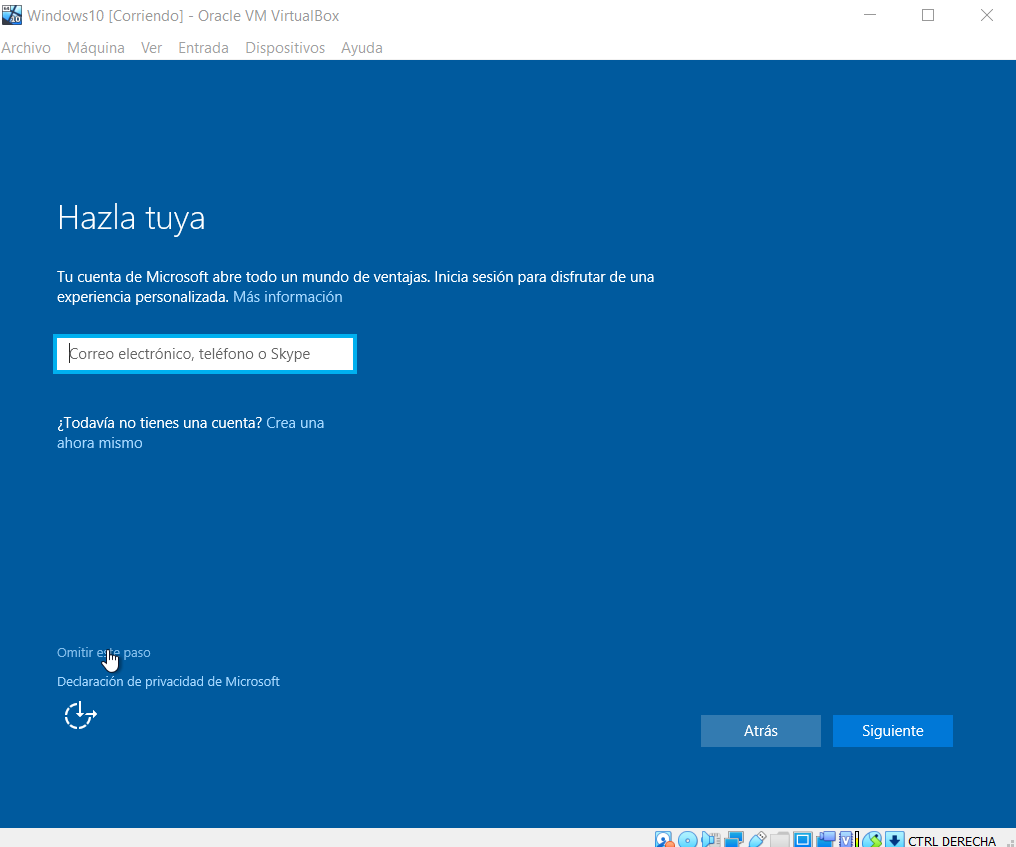
\includegraphics[scale = 0.4]{img/windows_install_21.png}
        \caption{Correo de cuenta Microsoft.}
        \label{Windows11}
      \end{figure}

      Despues de esto, nos pedirá el nombre de usuario y la contraseña para iniciar Windows, que sencilla mente es rellenar los campos.

      \begin{figure}[h]
        \centering
        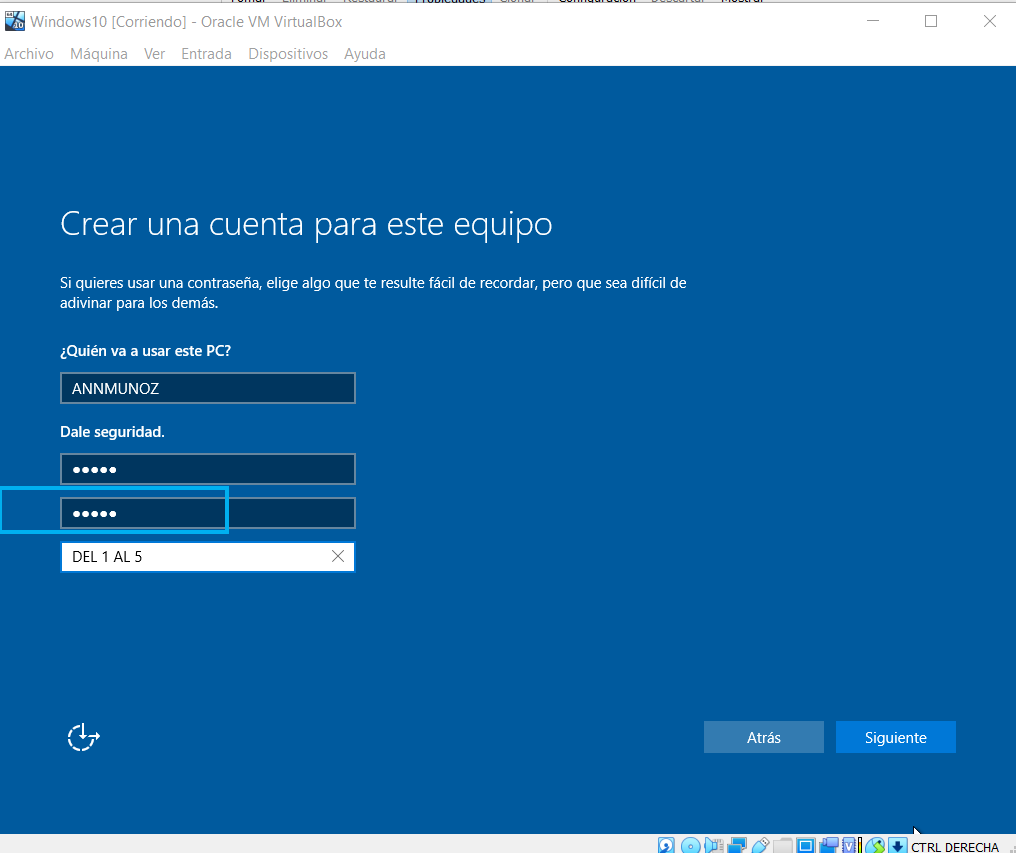
\includegraphics[scale = 0.4]{img/windows_install_22.png}
        \caption{Creación de usuario.}
        \label{Windows12}
      \end{figure}

      Una vez rellenado, la instalación estará acabada.

      \newpage

      Para comprobar las actualizaciones nos vamos a \textit{Configuracion -> Actualizaciones y Seguridad -> Windows Update}

      \begin{figure}[h]
        \centering
        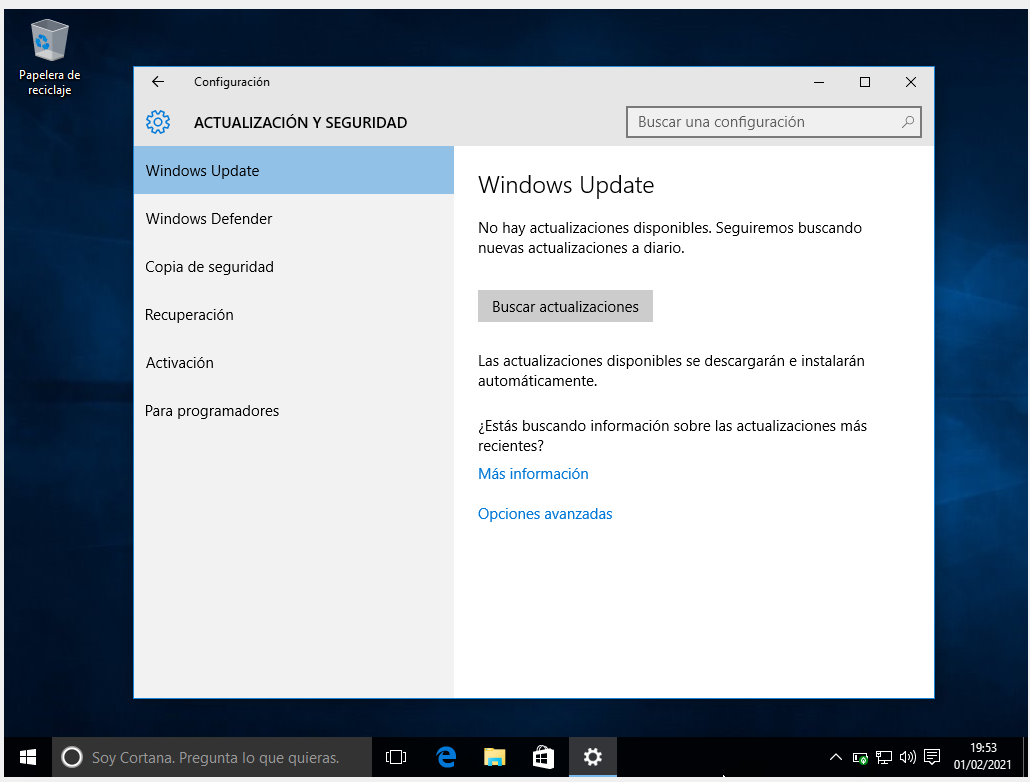
\includegraphics[scale = 0.5]{img/windows_install_24.png}
        \caption{Actualizaciones.}
        \label{Windows13}
      \end{figure}


    \newpage

    \section{IMÁGENES}
    \listoffigures
      
\end{document}